\section{User Flow}
\label{sec:UF}

In questa sezione sono rappresentati i principali percorsi utente attraverso le funzionalità del sistema. Ogni user flow indica i requisiti, gli use case e le user story a cui contribuisce e mostra le principali decisioni e transizioni dal punto di vista dell'utente, senza introdurre dettagli tecnici di implementazione. I diagrammi sono generati dai sorgenti PlantUML conservati in \texttt{img/src} e adottano la notazione dei diagrammi di attività: il cerchio pieno indica l'inizio, i rettangoli arrotondati le azioni, i rombi le decisioni e il cerchio bordato la fine. Le etichette delle transizioni esprimono le condizioni dal punto di vista dell'utente.

% ---------------------------------------------------------------- UF-01
\UF{Consultazione dei dati di catalogo e importazione da CSV} \label{uf:dati}
Associato alle user story \USref{us:edifici}, \USref{us:mappa}, \USref{us:interventi}, \USref{us:import} e ai requisiti funzionali \RFref{rf:catalogo_edifici}, \RFref{rf:mappa}, \RFref{rf:catalogo_interventi}, \RFref{rf:filtri_interventi}, \RFref{rf:import_csv}; use case UC-01--UC-04.

\begin{figure}[H]
    \centering
    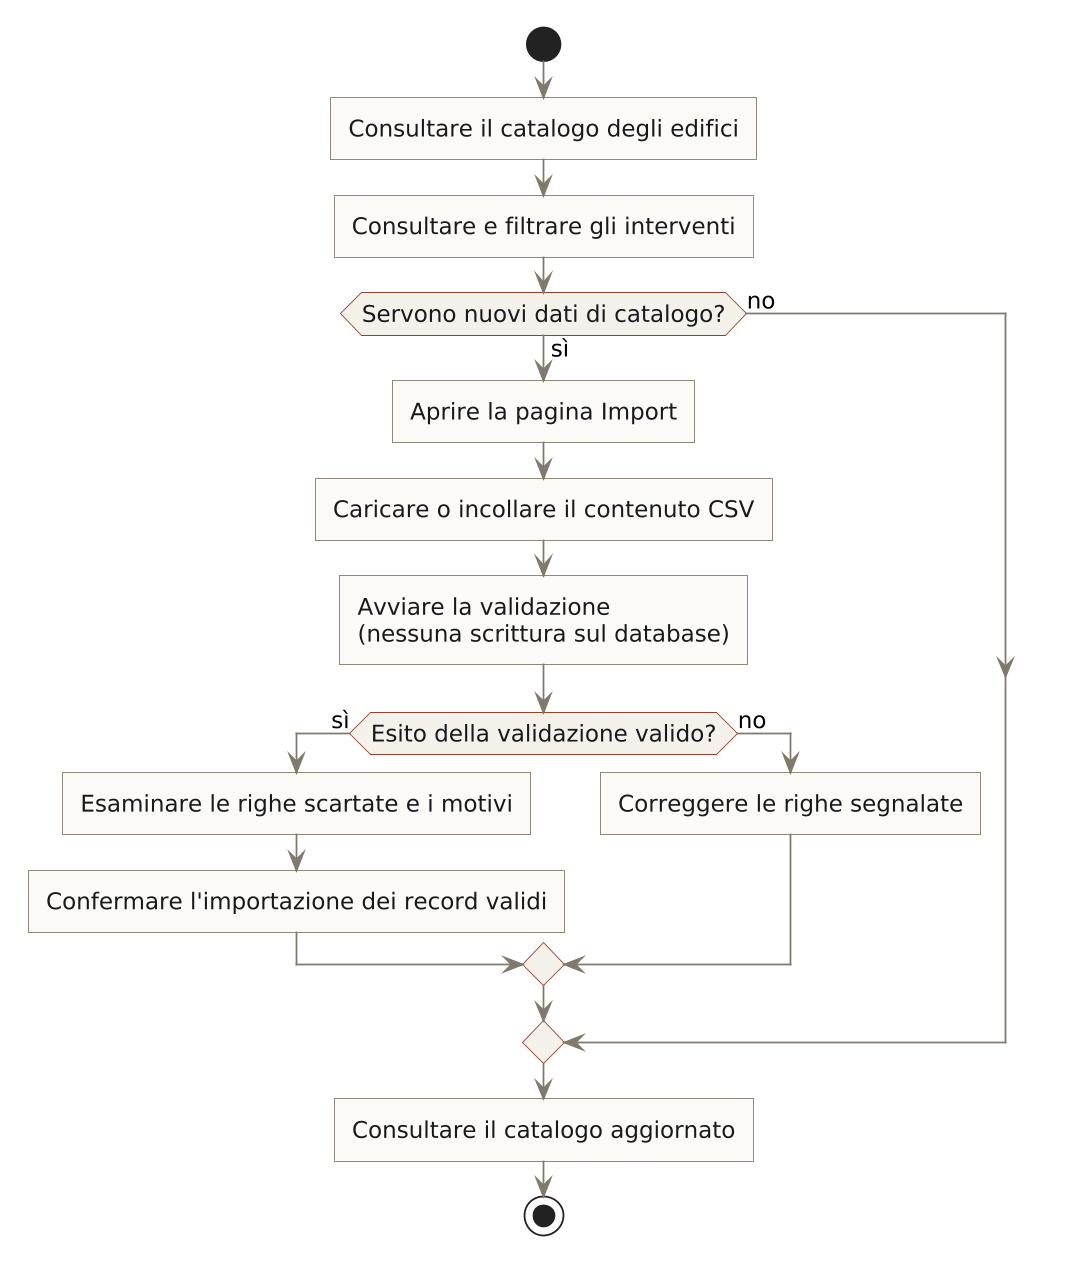
\includegraphics[height=0.52\textheight,keepaspectratio]{img/uf-01-dati.png}
    \caption{UF-01 --- Consultazione dei dati di catalogo e importazione da CSV.}
    \label{figuf:dati}
\end{figure}

La Figura~\ref{figuf:dati} mostra il percorso di consultazione del catalogo e di importazione. L'utente consulta edifici e interventi, applica filtri e, se servono nuovi dati, apre la pagina di importazione: la validazione non modifica il database e l'importazione viene confermata solo dopo aver esaminato le righe scartate. Il flusso termina con la consultazione del catalogo aggiornato.

% ---------------------------------------------------------------- UF-02
\UF{Configurazione dello scenario, proposta AI e approvazione umana} \label{uf:scenario}
Associato alle user story \USref{us:scenario}, \USref{us:vincoli}, \USref{us:ai}, \USref{us:ai_appr} e ai requisiti funzionali \RFref{rf:config_scenario}, \RFref{rf:candidati}, \RFref{rf:vincoli_scenario}, \RFref{rf:ai_proposta}, \RFref{rf:ai_approvazione}; use case UC-05, UC-06, UC-13, UC-14.

\begin{figure}[H]
    \centering
    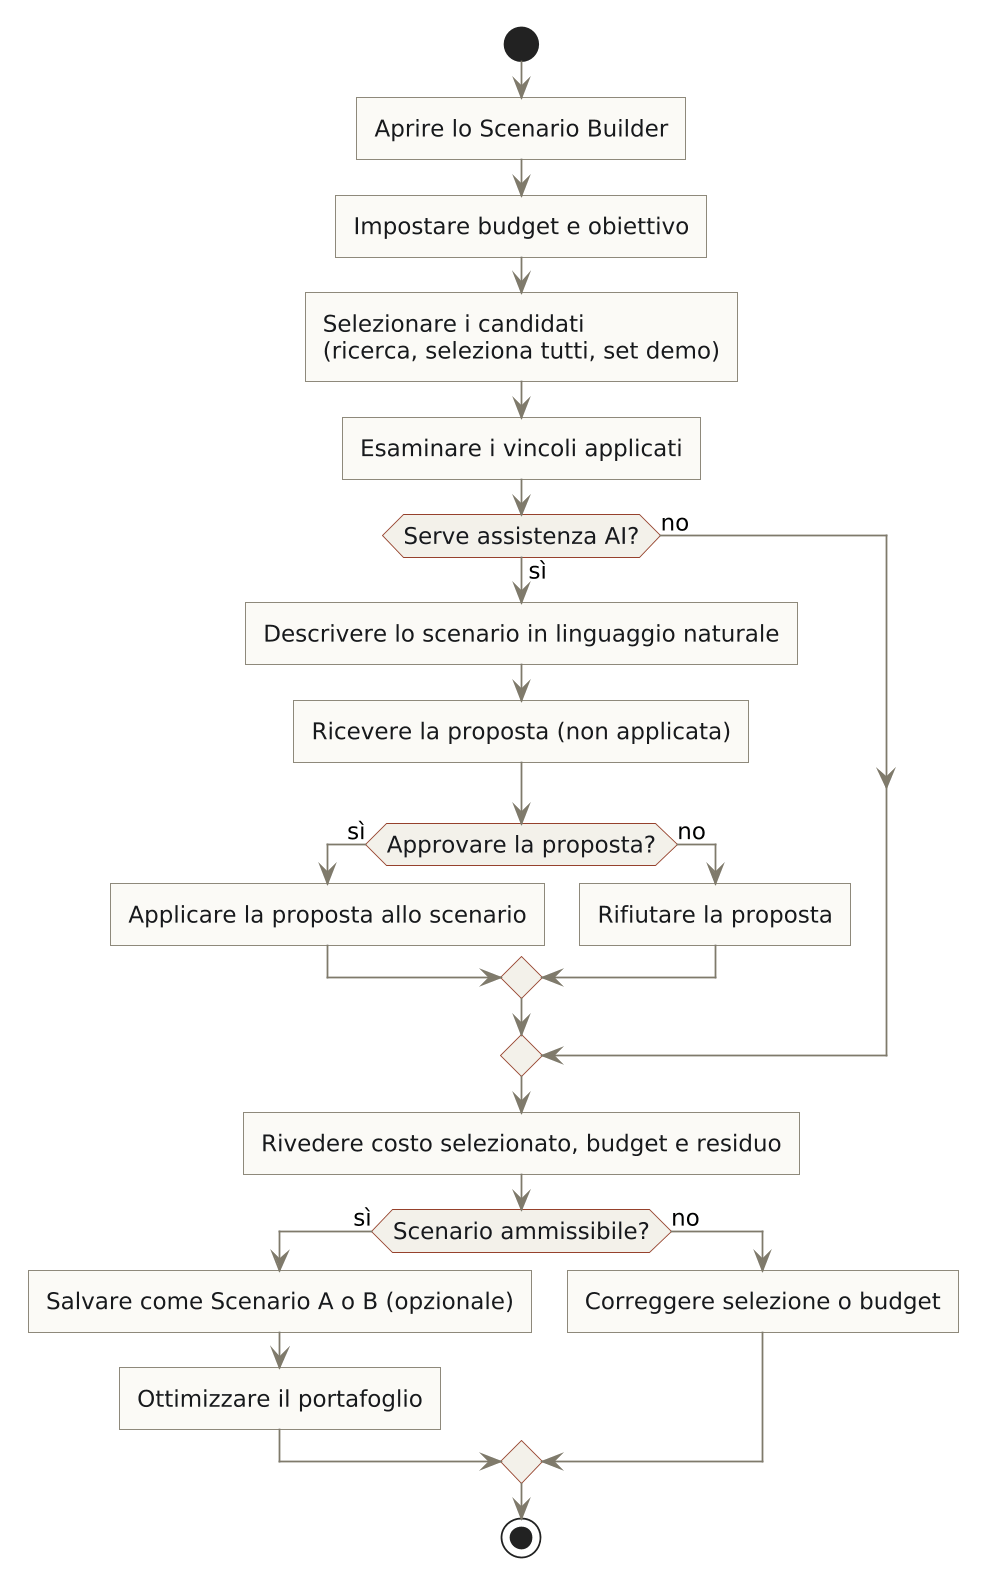
\includegraphics[height=0.62\textheight,keepaspectratio]{img/uf-02-scenario.png}
    \caption{UF-02 --- Configurazione dello scenario, proposta AI e approvazione umana.}
    \label{figuf:scenario}
\end{figure}

La Figura~\ref{figuf:scenario} mostra il percorso principale dell'operatore tecnico, dalla configurazione dello scenario alla richiesta di ottimizzazione. Il flusso esplicita il punto di approvazione umana della proposta AI: la proposta non viene mai applicata automaticamente, e anche dopo l'applicazione è l'utente a decidere se eseguire il solver.

% ---------------------------------------------------------------- UF-03
\UF{Esecuzione dell'ottimizzazione, dossier e stampa della relazione} \label{uf:ottimizzazione}
Associato alle user story \USref{us:ottimizza}, \USref{us:risultato}, \USref{us:spiegazioni}, \USref{us:tema} e ai requisiti funzionali \RFref{rf:ottimizzazione}, \RFref{rf:risultati}, \RFref{rf:spiegazioni}, \RFref{rf:tema}; use case UC-07, UC-08, UC-15.

\begin{figure}[H]
    \centering
    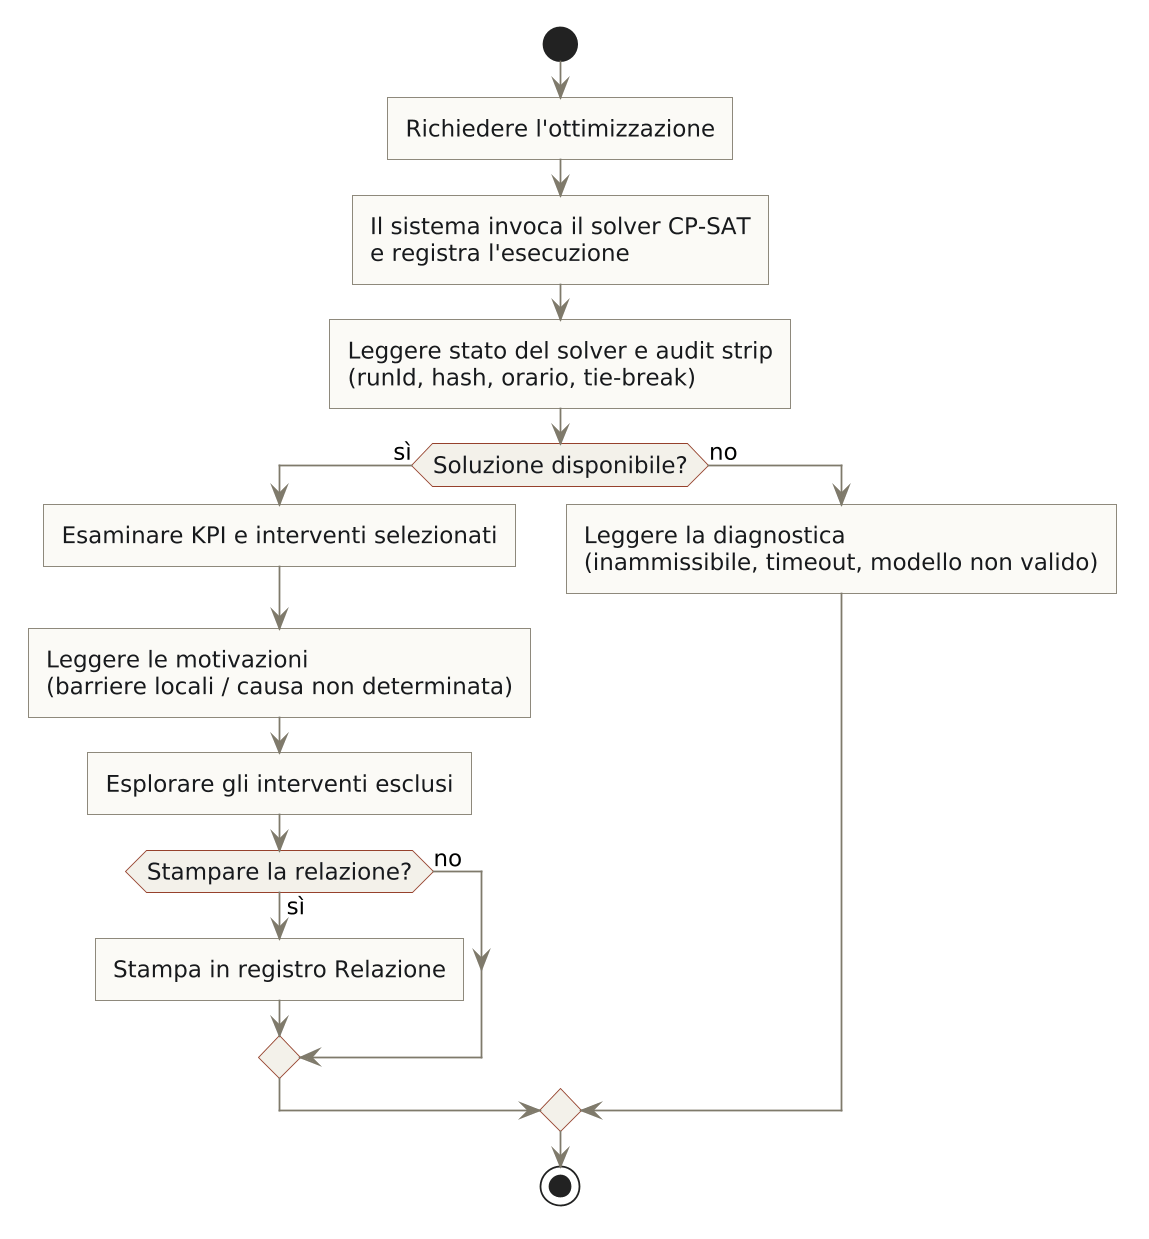
\includegraphics[height=0.55\textheight,keepaspectratio]{img/uf-03-ottimizzazione.png}
    \caption{UF-03 --- Esecuzione dell'ottimizzazione, lettura del dossier e stampa.}
    \label{figuf:ottimizzazione}
\end{figure}

La Figura~\ref{figuf:ottimizzazione} mostra il percorso di esecuzione dell'ottimizzazione e di lettura del dossier: l'utente richiede il calcolo, legge lo stato del solver e la fascia di audit, consulta gli interventi selezionati e le motivazioni, esplora le esclusioni e, se serve, stampa la relazione con fondo chiaro e inchiostro scuro. In caso di esito non risolutivo il flusso conduce alla diagnostica invece che a un portafoglio presentato come definitivo.

% ---------------------------------------------------------------- UF-04
\UF{Costruzione di alternative A/B, confronto e what-if} \label{uf:confronto}
Associato alle user story \USref{us:salva_ab}, \USref{us:confronto} e ai requisiti funzionali \RFref{rf:scenari_salvati}, \RFref{rf:confronto}; use case UC-10, UC-11.

\begin{figure}[H]
    \centering
    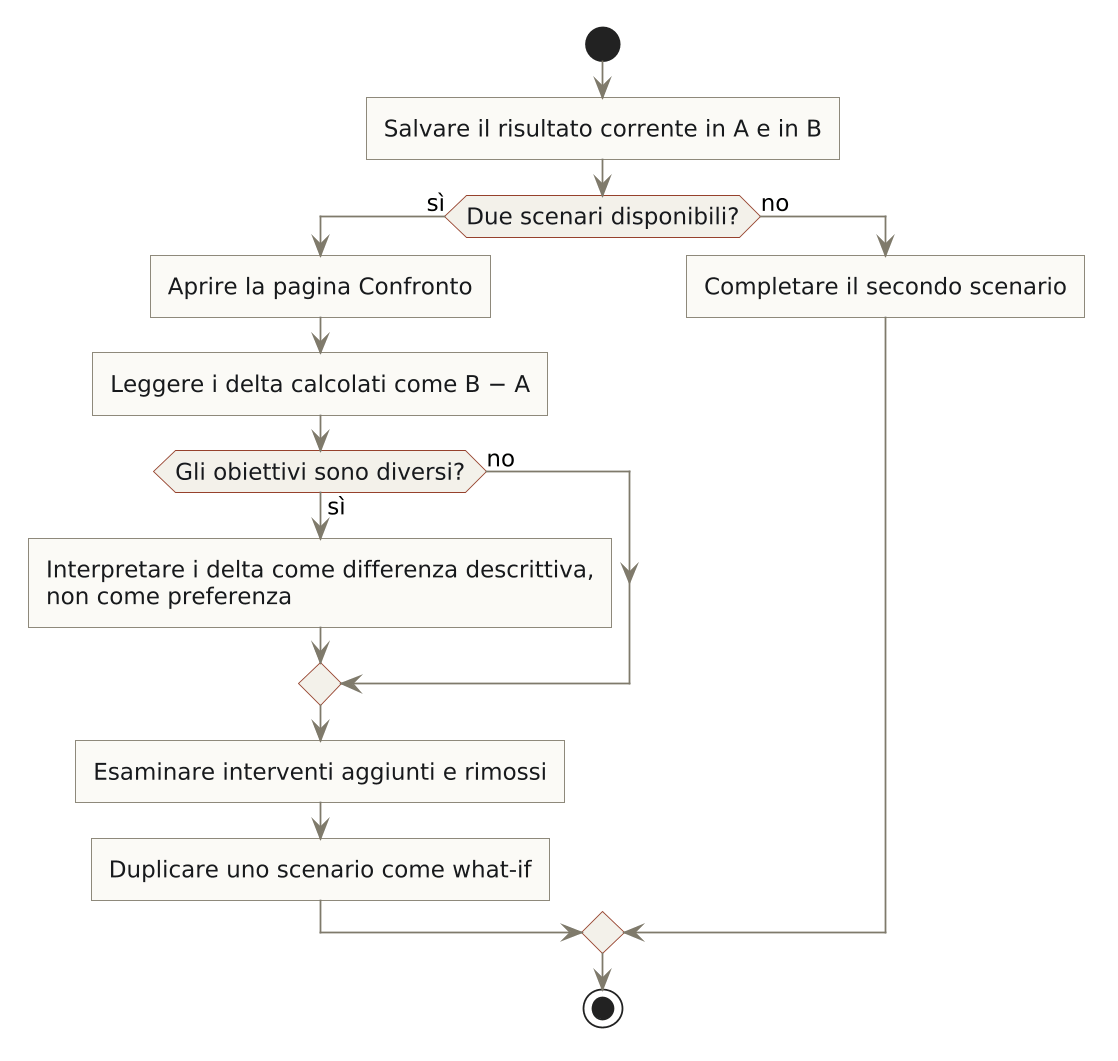
\includegraphics[height=0.52\textheight,keepaspectratio]{img/uf-04-confronto.png}
    \caption{UF-04 --- Costruzione delle alternative A/B, confronto e what-if.}
    \label{figuf:confronto}
\end{figure}

La Figura~\ref{figuf:confronto} mostra il percorso di costruzione di due alternative e del loro confronto. L'utente salva i risultati negli slot A e B, legge gli scostamenti calcolati come $B - A$, verifica l'eventuale non omogeneità degli obiettivi, esamina gli interventi aggiunti e rimossi e può duplicare uno scenario come what-if per costruire una terza alternativa. Il decisore comunale è il tipico fruitore finale di questa vista.

% ---------------------------------------------------------------- UF-05
\UF{Analisi di sensibilità sul budget} \label{uf:sensibilita}
Associato alla user story \USref{us:sensibilita} e al requisito funzionale \RFref{rf:sensibilita}; use case UC-12.

\begin{figure}[H]
    \centering
    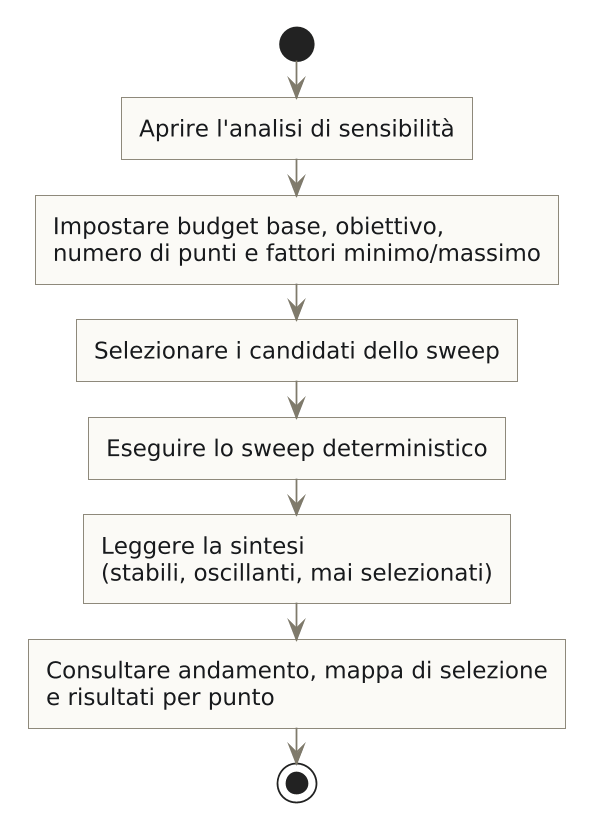
\includegraphics[height=0.48\textheight,keepaspectratio]{img/uf-05-sensibilita.png}
    \caption{UF-05 --- Analisi di sensibilità sul budget.}
    \label{figuf:sensibilita}
\end{figure}

La Figura~\ref{figuf:sensibilita} mostra il percorso di analisi di sensibilità: definizione della griglia di budget, selezione dei candidati, esecuzione dello sweep deterministico e lettura della sintesi con la classificazione delle opzioni in sempre selezionate, oscillanti e mai selezionate. La nota metodologica chiarisce che l'analisi non è una simulazione Monte Carlo e che varia il solo parametro budget.
